
%(BEGIN_QUESTION)
% Copyright 2006, Tony R. Kuphaldt, released under the Creative Commons Attribution License (v 1.0)
% This means you may do almost anything with this work of mine, so long as you give me proper credit

To trykkdrevne «løftere» brukes for å løfte en tung last fra bakken. Den ene løfteren bruker olje under trykk (fra en hydraulikkpumpe), mens den andre bruker luft under trykk (fra en luftkompressor). Hver løfter har en stengeventil i linjen som mater fluid til sylinderen, slik at stempelbevegelsen kan stoppes:

$$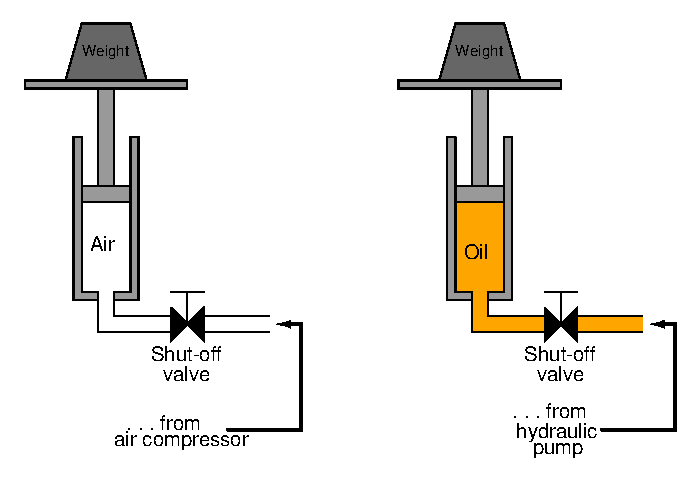
\includegraphics[width=15.5cm]{i00750x01.eps}$$

Hva vil skje dersom lasten faller av løfteplattformen etter at den er hevet fra bakken, i hvert av tilfellene? Anta at stengeventilen er lukket (ingen fluidstrøm fra pumpe eller kompressor til sylinderen) når dette skjer.

\vskip 20pt \vbox{\hrule \hbox{\strut \vrule{} {\bf Forslag til sokratisk diskusjon} \vrule} \hrule}

\begin{itemize}
\item{} Hvilke generelle lærdommer kan vi trekke fra dette eksempelet om sikkerhet ved trykksatte fluid?
\item{} Endres beregningen av stempelkraft basert på trykk ($F = PA$) hvis fluidet er en {\it gass} i stedet for en {\it væske}?
\end{itemize}

\underbar{file i00750}
%(END_QUESTION)





%(BEGIN_ANSWER)

Hvis lasten faller av den oljedrevne løfteren, vil stempelet holde sin opprinnelige posisjon. Hvis lasten faller av den luftdrevne løfteren, vil stempelet stige betydelig (kanskje til og med skytes helt ut av sylinderen!) på grunn av ekspansjon i luften:

$$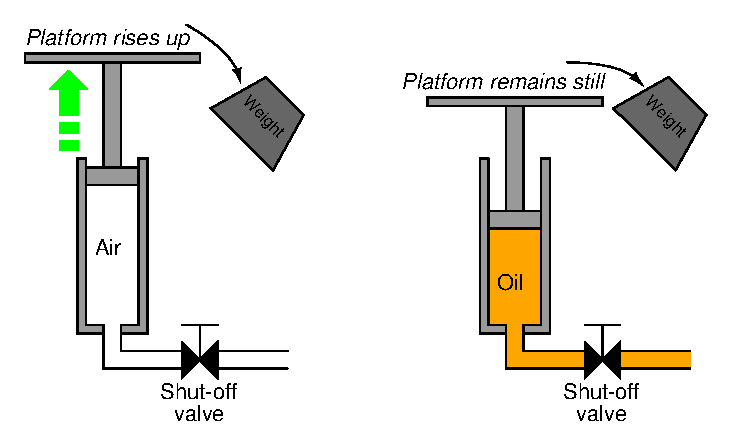
\includegraphics[width=15.5cm]{i00750x02.eps}$$

%(END_ANSWER)





%(BEGIN_NOTES)

Dette spørsmålet bygger på en hendelse fortalt av en tidligere medstudent: Han jobbet med montering av ventilasjonskanaler og brukte en luftdrevet løfter til å heise opp en stor kasse med platemetall og verktøy til et tak. Idet han løftet kassen av plattformen, skjøt plattformen og sylinderen opp, stempelet poppet helt ut av sylinderen og alt krasjet ned i bakgaten under. Heldigvis ble ingen skadet.

%INDEX% Mekanikk, fluidkraftsystemer: hydraulisk/pneumatisk billøfter
%INDEX% Fysikk, statiske væsker: kompressibilitet

%(END_NOTES)


